\section{Phân tích và Mô phỏng toàn vẹn tín hiệu và nguồn (Signal and Power Integrity Analysis and Simulation)}
    \subsection{Mô phỏng Toàn vẹn tín hiệu (Signal Integrity)}
        Việc mô phỏng được thực hiện trên các đường tín hiệu quan trọng để xác minh tính toán lý thuyết so với thiết kế layout thực tế.
        
        \begin{enumerate}
            \renewcommand{\labelenumi}{\alph{enumi}.}
            \item \textbf{Mô phỏng đường tín hiệu đơn cực (Single-ended Bus):}
            
            \begin{figure}[h]
                \centering
                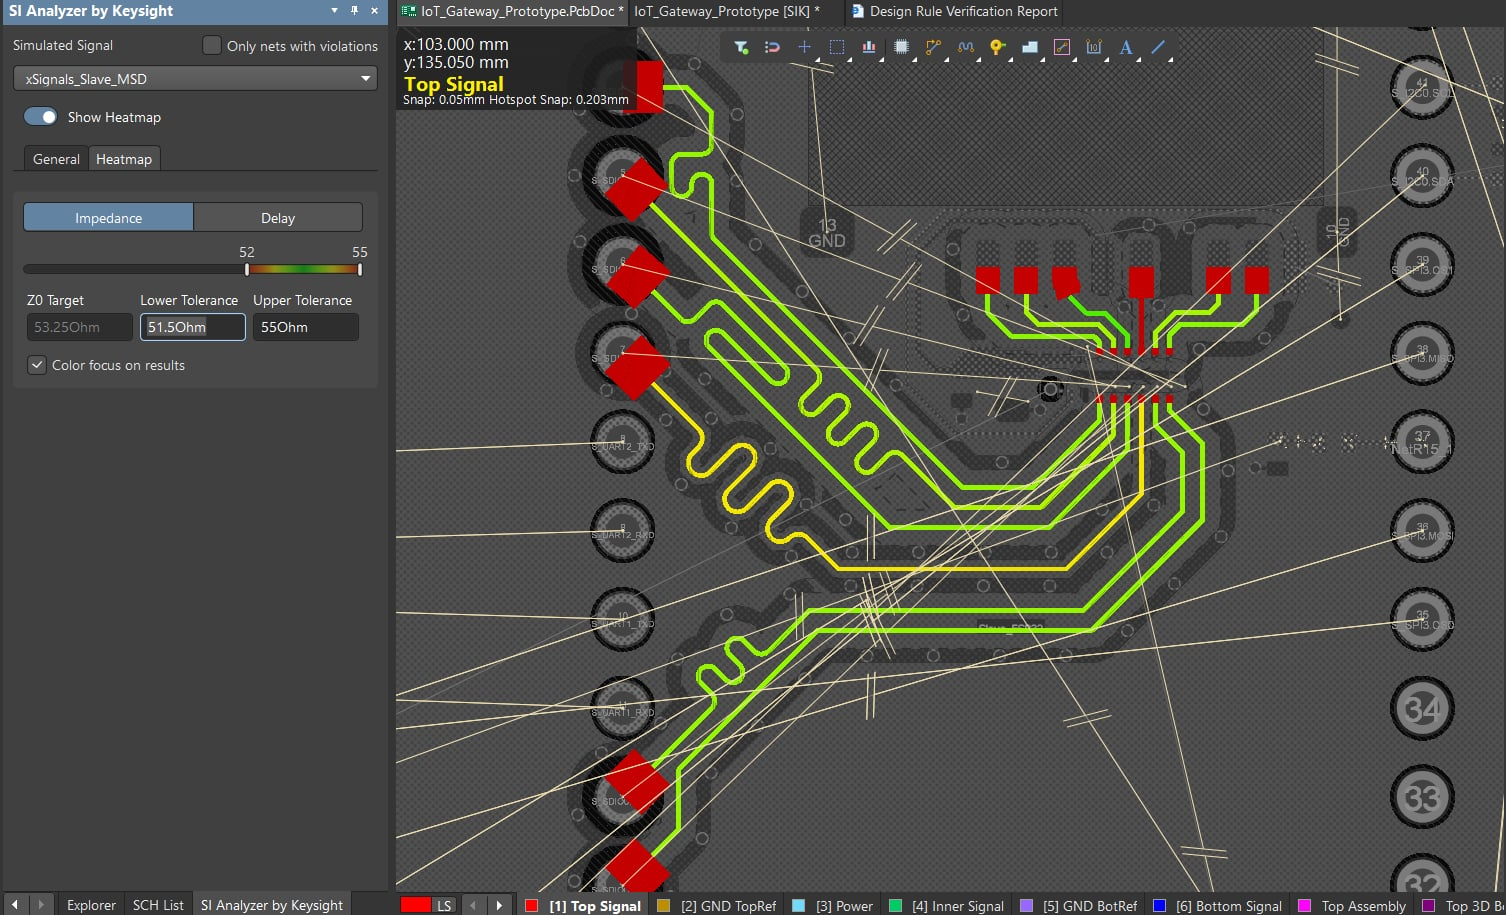
\includegraphics[width=0.5\textwidth]{figures/sdio_sim_impedance.jpg}
                \caption{Biểu đồ phân bố trở kháng (Impedance Heatmap) đường tín hiệu đơn cực.}
                \label{fig:sdio_impedance}
            \end{figure} 
            Kết quả mô phỏng cho thấy trở kháng đặc tính ($Z_0$) dao động trong khoảng từ $51.5\Omega$ đến $55\Omega$. Mức biến thiên này hoàn toàn nằm trong phạm vi dung sai thiết kế cho phép ($\pm 10\%$ so với mục tiêu $50\Omega$), đảm bảo phối hợp trở kháng tốt với các linh kiện chuẩn. Tuy có sự mismatch tại các pinout nhưng độ dài mismatch là đủ nhỏ để không ảnh hưởng quá lớn đến trở kháng chung.
            
            \begin{figure}[h]
                \centering
                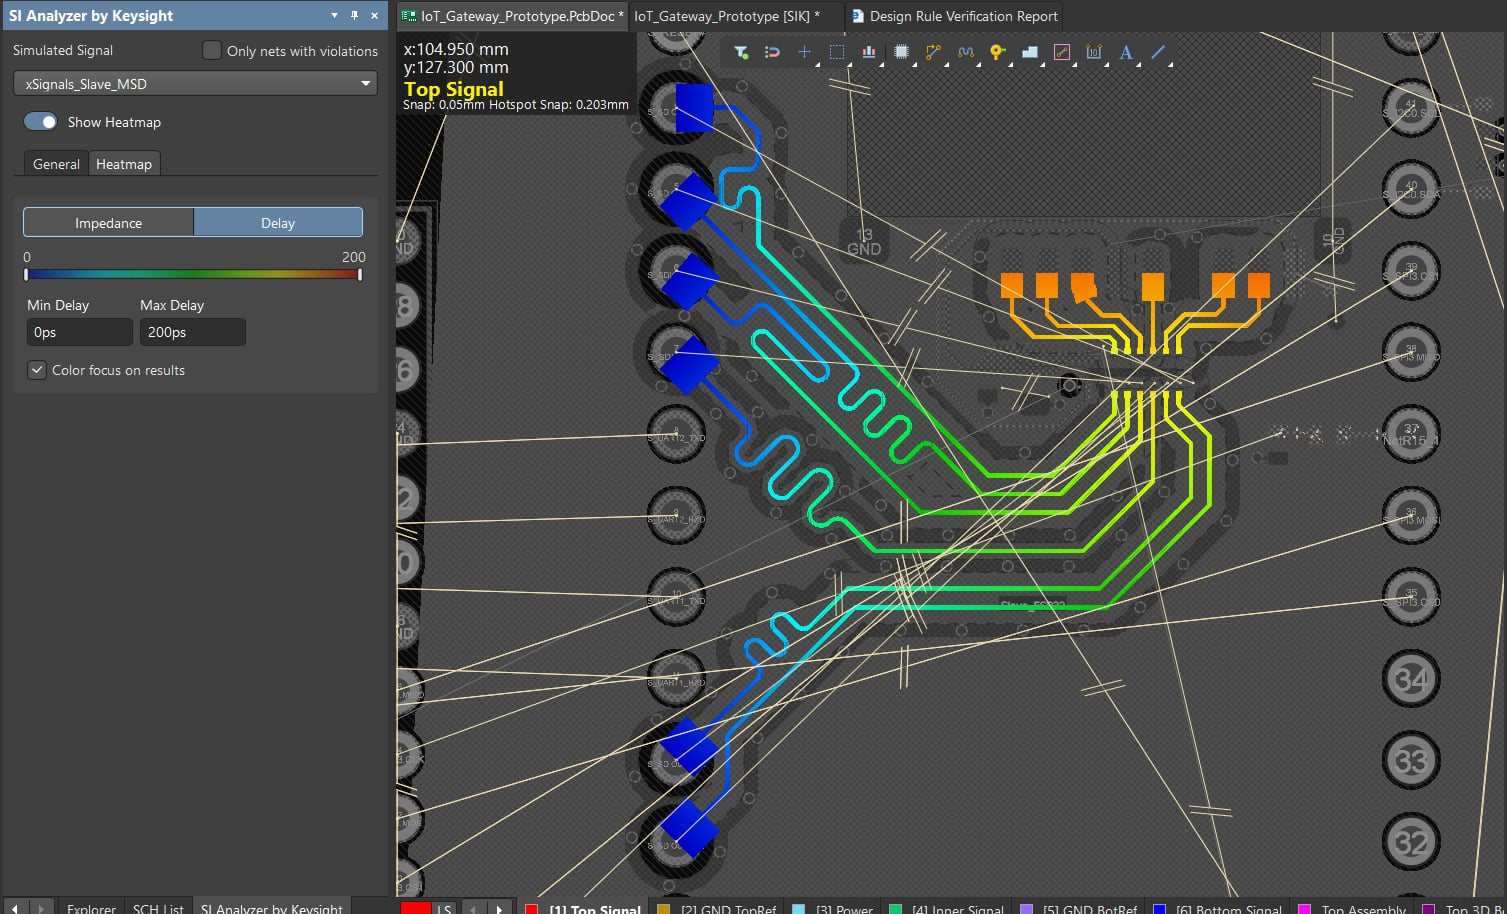
\includegraphics[width=0.5\textwidth]{figures/sdio_sim_delay.jpg}
                \caption{Biểu đồ phân bố độ trễ lan truyền (Propagation Delay) đường tín hiệu đơn cực.}
                \label{fig:sdio_delay}
            \end{figure} 
            Độ trễ lan truyền của toàn bộ các đường tín hiệu được kiểm soát dưới ngưỡng $200ps$. Sự đồng nhất của dải màu trên biểu đồ heatmap dọc theo chiều dài đường mạch cho thấy độ lệch pha giữa các tín hiệu là nhỏ, đảm bảo các bit dữ liệu đến đích đồng bộ với xung nhịp.
            
            \begin{figure}[h]
                \centering
                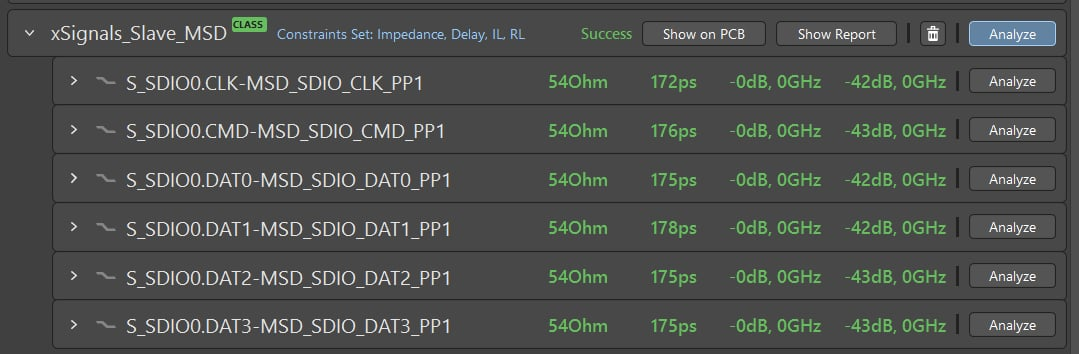
\includegraphics[width=0.6\textwidth]{figures/sdio_sim_report.jpg}
                \caption{Bảng tổng hợp thông số mô phỏng đường tín hiệu đơn cực.}
                \label{fig:sdio_report}
            \end{figure} 
            Số liệu chi tiết từ báo cáo xác nhận:
            \begin{itemize}
                \item Trở kháng trung bình đạt $54\Omega$.
                \item Độ trễ dao động trong biên độ hẹp ($175ps$ - $178ps$), cho thấy việc cân bằng chiều dài (Length matching) đã được thực hiện tốt.
                \item Tổn hao chèn (Insertion Loss) gần như bằng $0dB$ và Tổn hao phản xạ (Return Loss) đạt $-42dB$ (rất thấp), chứng tỏ năng lượng tín hiệu được truyền đi hiệu quả và phản xạ tại tải là không đáng kể.
            \end{itemize}


            \item \textbf{Mô phỏng cặp tín hiệu vi sai (Differential-pair):}
            
            \begin{figure}[h]
                \centering
                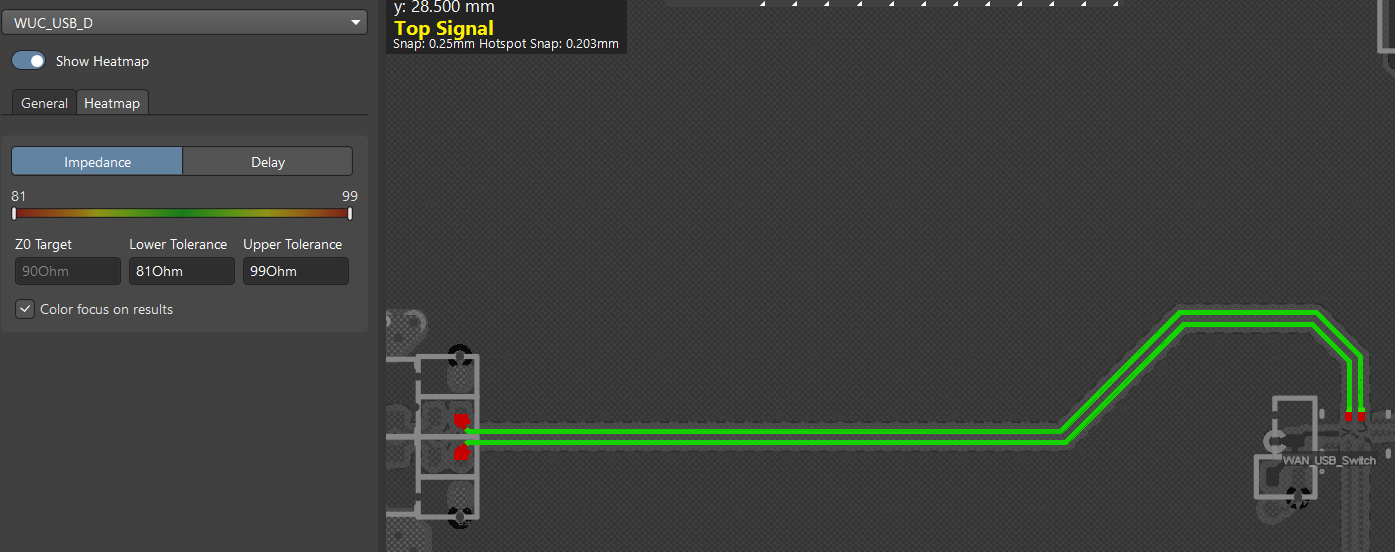
\includegraphics[width=0.5\textwidth]{figures/usb_sim_impedance.png}
                \caption{Biểu đồ phân bố trở kháng (Impedance Heatmap) đường vi sai.}
                \label{fig:usb_impedance}
            \end{figure} 
            Trở kháng vi sai ($Z_{diff}$) mô phỏng đạt giá trị ổn định quanh mức $90\Omega$. Kết quả này tuân thủ chặt chẽ tiêu chuẩn yêu cầu $90\Omega \pm 10\%$.  Tuy có sự mismatch tại các pinout nhưng độ dài mismatch là đủ nhỏ để không ảnh hưởng quá lớn đến trở kháng chung.
            
            \begin{figure}[h]
                \centering
                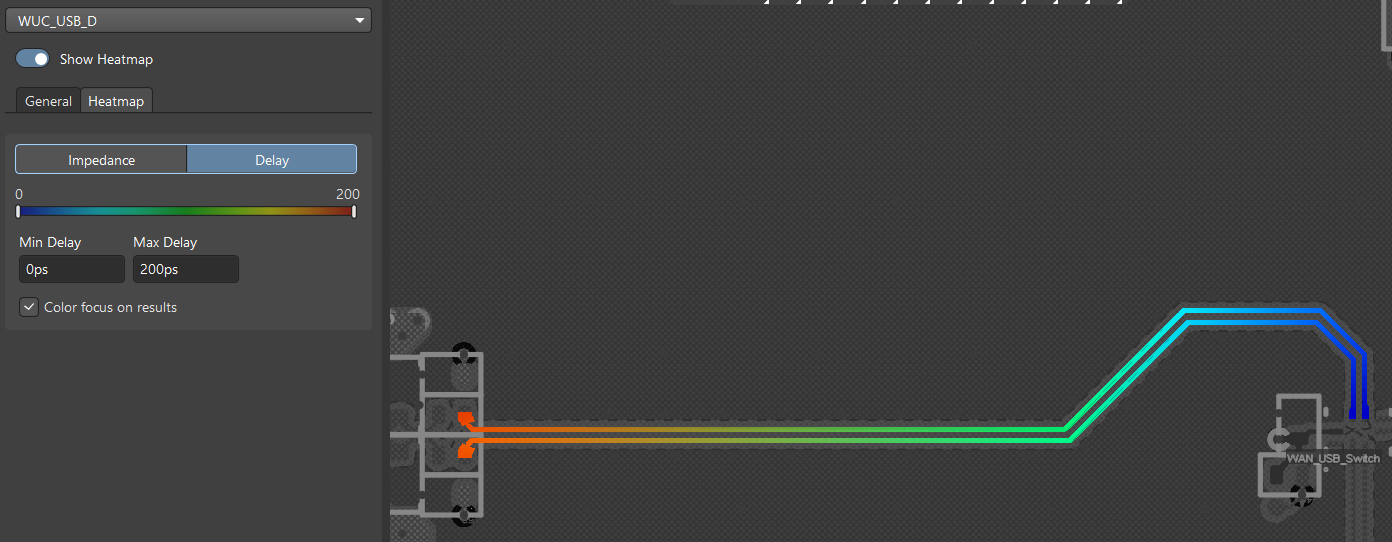
\includegraphics[width=0.5\textwidth]{figures/usb_sim_delay.png}
                \caption{Biểu đồ phân bố độ trễ lan truyền (Propagation Delay) đường vi sai.}
                \label{fig:usb_delay}
            \end{figure} 
            Thời gian độ trễ lan truyền được duy trì dưới $200ps$. Sự tương đồng về màu sắc trên hai nhánh D+ và D- khẳng định độ lệch pha là nhỏ, giúp triệt tiêu hiệu quả nhiễu chế độ chung (Common Mode Noise).
            
            \begin{figure}[h]
                \centering
                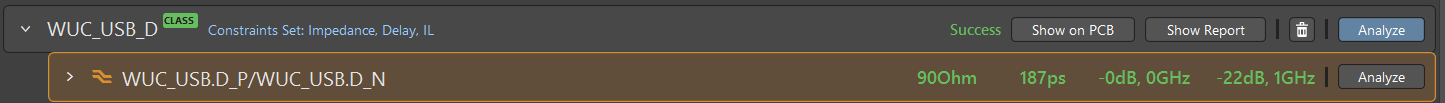
\includegraphics[width=0.6\textwidth]{figures/usb_sim_report.png}
                \caption{Bảng tổng hợp thông số mô phỏng đường vi sai.}
                \label{fig:usb_report}
            \end{figure} 
            Kết quả tổng hợp cho thấy:
            \begin{itemize}
                \item Trở kháng vi sai đạt chuẩn $90\Omega$.
                \item Độ trễ đường truyền là $187ps$.
                \item Các thông số S-parameter rất tích cực: Insertion Loss xấp xỉ $0dB$ và Return Loss đạt $-22dB$, đảm bảo tính toàn vẹn tín hiệu cho giao tiếp dữ liệu tốc độ cao.
            \end{itemize}      
        \end{enumerate}

    \subsection{Mô phỏng Toàn vẹn nguồn (Power Integrity)}
        \subsubsection{Sơ đồ Cây phân phối nguồn (Power Tree)}
            Hệ thống được thiết kế thành cấu trúc nguồn phân tầng đa nhánh phức tạp, được thể hiện trong \autoref{fig:power_tree}. Mạng lưới này không chỉ đơn thuần là cấp điện, mà là một hệ thống quản lý năng lượng phân tán với nhiều đặc điểm kỹ thuật cần phải đảm bảo trong thiết kế Mạng phân phối nguồn (Power Distribution Network - PDN).

            \begin{figure}[h]
                \centering
                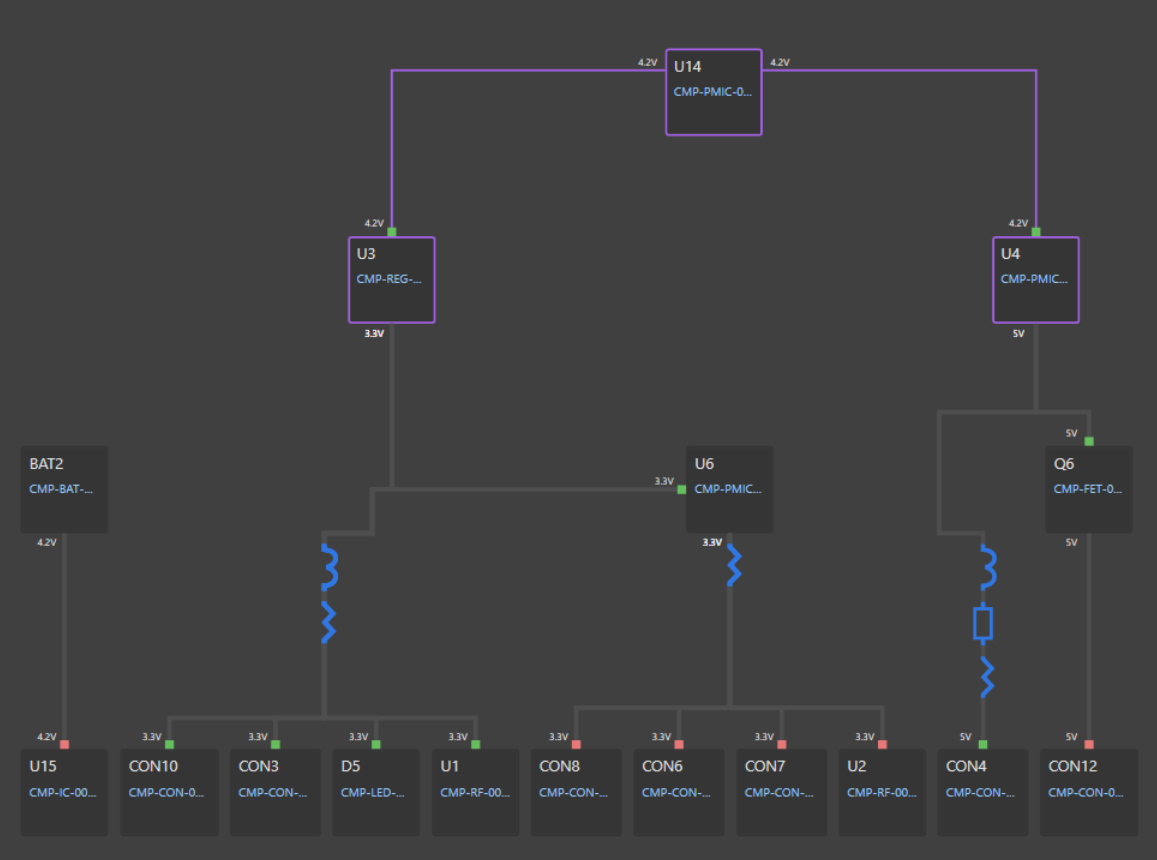
\includegraphics[width=0.6\textwidth]{figures/power_tree.png}
                \caption{Cấu trúc mạng phân phối nguồn.}
                \label{fig:power_tree}
            \end{figure}
            
            Với cấu trúc chằng chịt và dòng tải biến động lớn, việc tính toán lý thuyết và thực hiện Mô phỏng PDN để kiểm chứng độ sụt áp (DC IR Drop) và mật độ dòng điện (Current Density), đảm bảo không xảy ra quá nhiệt cục bộ hoặc sụt áp vượt ngưỡng an toàn.\par
            \newpage
            Dựa trên thiết kế, mô phỏng tập trung vào các ray nguồn quan trọng ở trạng thái tải ước tính là $20\%$ công suất lý thuyết\footnote{Đây là giá trị được tính toán để đảm bảo mức tiêu thụ điện thấp, xem trong phần ???}, bao gồm các nguồn có tải cao:
            \begin{itemize}
                \item Nguồn +4V2\_VSYS (nguồn U14)
                \item Nguồn +5V0\_CTRL (nguồn U4)
                \item Nguồn +3V3 (nguồn U3)
                \item Nguồn +3V3\_CTRL (nguồn U6)
                \item Nguồn +3V7\_BAT (nguồn BAT2)
            \end{itemize}

        \subsubsection{Phân tích và Mô phỏng Mật độ dòng điện}
            
            Mục tiêu của quá trình mô phỏng là xác minh tính toàn vẹn của mạng phân phối nguồn (PDN) dưới điều kiện tải lý thuyết ($20\%$ công suất tối đa). Mật độ dòng điện quá lớn có thể gây hư hỏng mạch và sụt áp quá nhiều sẽ dẫn đến hiệu suất kém hoặc thậm chí không hoạt động. Do đó, việc phân tích kỹ lưỡng các ray nguồn chính là rất quan trọng để đảm bảo thiết kế đáp ứng các tiêu chí kỹ thuật đã đề ra.

            \textbf{Tính toán các giá trị điều kiện mô phỏng:}\\
            Mật độ dòng điện ảnh hưởng đến khả năng tải dòng và mức tăng nhiệt độ theo công thức $I = k\Delta T^{0.44}A^{0.725}$, trong đó\cite{PrintedBoardDesignIpc2221A}:
            \begin{itemize}
                \item $I$: Dòng điện (A)
                \item $\Delta T$: Mức tăng nhiệt độ (°C)
                \item $A$: Tiết diện mặt cắt ngang của đường dây (sq.mils)  
                \item $k$: Hằng số điều chỉnh:
                \begin{itemize}
                    \item $k = 0.048$ cho lớp ngoài (Outer layer).
                    \item $k = 0.024$ cho lớp trong (Inner layer).
                \end{itemize}
            \end{itemize}
            
            Tiết diện mặt cắt $A = w \times t$, trong đó $w$ là chiều rộng và $t$ là chiều dày của đường dây. Độ dày lớp ngoài là 0.035mm và lớp trong là 0.0152mm.\\
            Xét mức tăng nhiệt độ $\Delta T$ an toàn là $20^{\circ}C$\\
            Khảo sát các độ rộng đường dây trong quá trình layout để tính ra mật độ dòng điện $J = \dfrac{I}{A}$\\

            \begin{longtable}{|c|c|c|}
                \caption{Bảng khảo sát mật độ dòng điện}\\
                \hline
                Độ rộng đường dây & Lớp ngoài & Lớp trong \\
                \hline
                \endfirsthead
                
                \hline
                Độ rộng đường dây & Lớp ngoài & Lớp trong \\
                \hline
                \endhead
                
                \hline
                \endfoot
                
                \hline
                \endlastfoot
                
                1.0mm & 92.7 A/mm$^2$ & 58.3 A/mm$^2$ \\
                1.5mm & 82.9 A/mm$^2$ & 52.1 A/mm$^2$ \\
                2.0mm & 76.6 A/mm$^2$ & 48.1 A/mm$^2$ 
                \label{tab:current_density_survey}\\

                \hline
            \end{longtable}

            \textbf{Tiêu chí chấp nhận:} Trong quá trình layout, các đường dẫn thường sẽ lớn hơn 1mm, từ bảng khảo sát có thể giới hạn mật độ dòng điện tối đa cho lớp ngoài là 90 A/mm$^2$ và lớp trong là 50 A/mm$^2$. Các giá trị này được sử dụng làm cơ sở để đánh giá kết quả mô phỏng mật độ dòng điện và sụt áp DC trên các ray nguồn chính.

            \begin{enumerate}
                \item \textbf{Phân tích Ray nguồn +4V2\_VSYS:}
                    
                    Mô phỏng được thực hiện với dòng tải lý thuyết là $I_{load} = 0.95A$ theo mạng nguồn trong \autoref{fig:4v2_vsys_power_tree}.

                    \begin{figure}[h]
                        \begin{minipage}{0.3\textwidth}
                            \vspace{0pt}
                            Trong đó:
                            % \begin{itemize}
                            %     \item U15 là nguồn BQ25892RTWR với trở kháng đầu ra là $27 \text{m}\Omega$\cite{FastChargerBq2589x}.
                            %     \item U3 là tải TPS566231RQFR với điện áp đầu vào tối thiểu là 3.0V\cite{StepDownRegulatorTps56623x}.
                            %     \item U4 là tải TPS22965DSGR với điện áp đầu vào tối thiểu là 2.5V\cite{LoadSwitchTps22965}.
                            % \end{itemize}
                            awdha uwiudh awiud aiuhw iudawih iudaawdha uwiudh awiud aiuhw iudawih iudaawdha uwiudh awiud aiuhw iudawih iudaawdha uwiudh awiud aiuhw iudawih iudaawdha uwiudh awiud aiuhw iudawih iudaawdha uwiudh awiud aiuhw iudawih iudaawdha uwiudh awiud aiuhw iudawih iudaawdha uwiudh awiud aiuhw iudawih iudaawdha uwiudh awiud aiuhw iudawih iudaawdha uwiudh awiud aiuhw iudawih iudaawdha uwiudh awiud aiuhw iudawih iudaawdh
                        \end{minipage}

                        \hfill
                        \begin{minipage}{0.3\textwidth}
                            \centering
                            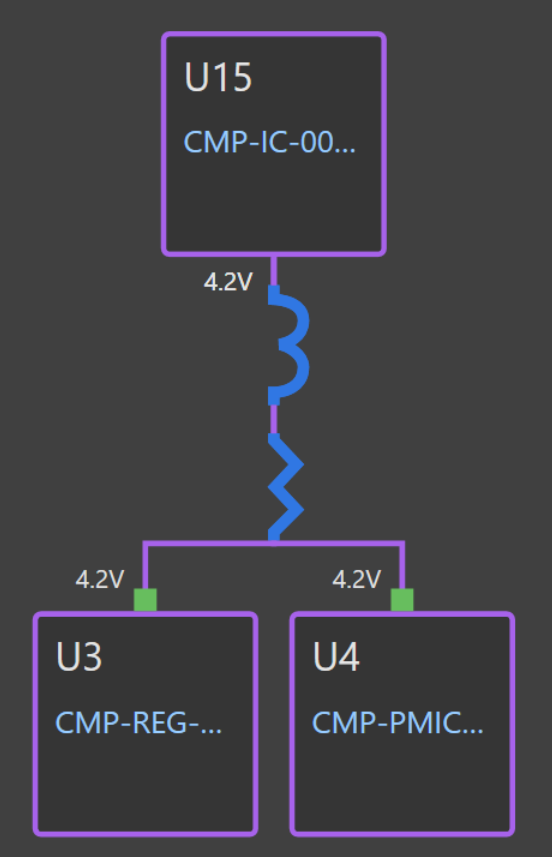
\includegraphics[width=0.5\textwidth]{figures/4v2_vsys_power_tree.png}
                            \caption{Cây phân phối nguồn +4V2\_VSYS.}
                            \label{fig:4v2_vsys_power_tree}
                        \end{minipage}
                    \end{figure}

                    \begin{figure}[h]
                        \centering
                        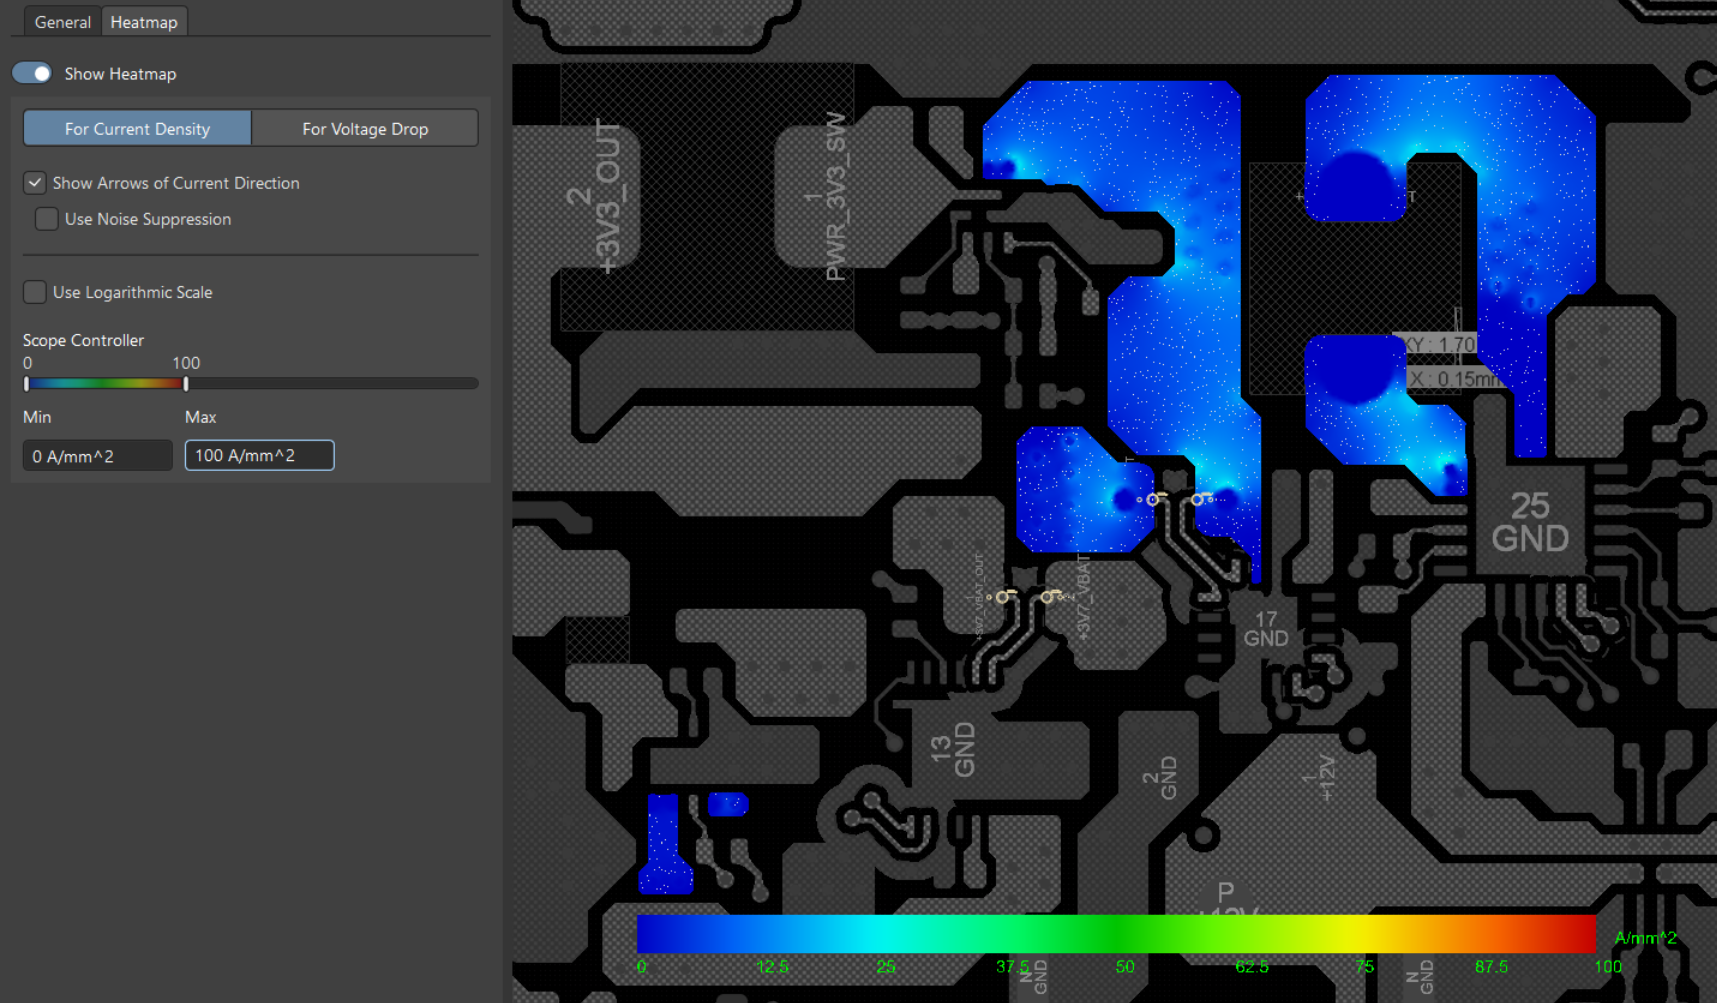
\includegraphics[width=0.45\textwidth]{figures/4v2_vsys_sim_current_density_outer.png}
                        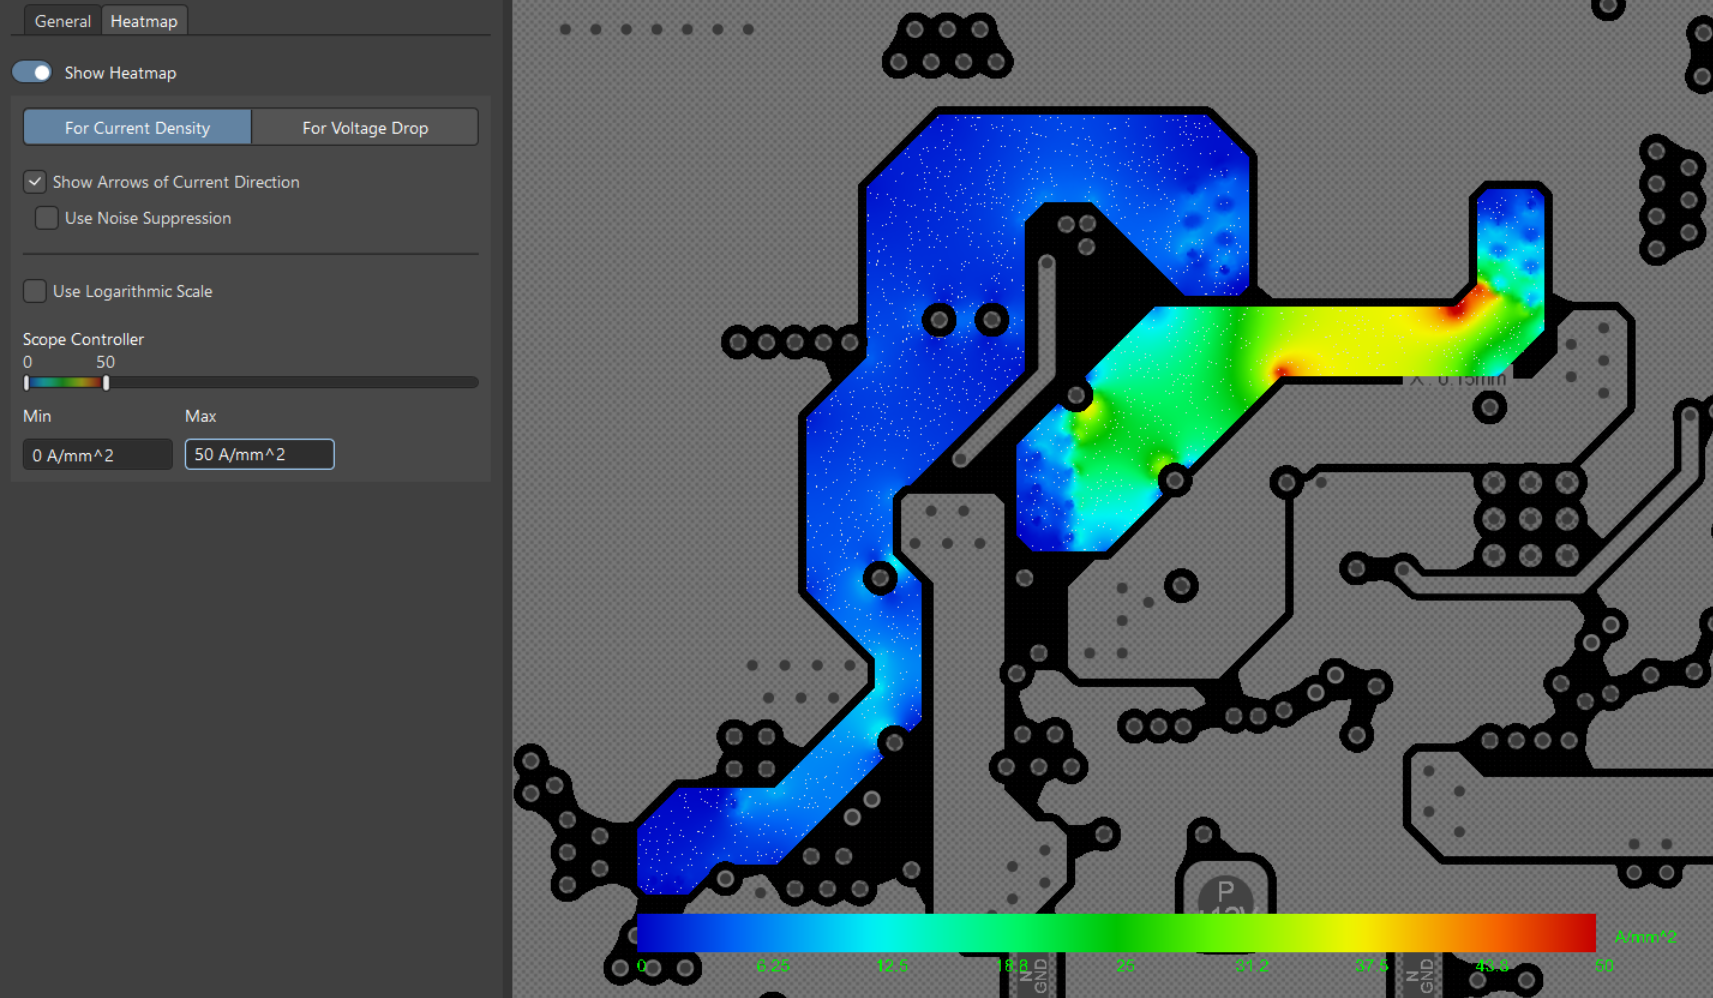
\includegraphics[width=0.45\textwidth]{figures/4v2_vsys_sim_current_density_inner.png}
                        \caption{Biểu đồ phân bố mật độ dòng điện của nguồn +4V2\_VSYS.}
                        \label{fig:4v2_vsys_current_density}
                    \end{figure}

                    \textbf{\textit{Kết quả mô phỏng Mật độ dòng điện:}}\\
                    Trên tổng thể toàn bộ đường dây vẫn đạt được mật độ dòng điện an toàn, tuy nhiên vẫn có một số điểm tập trung dòng cao nhất đạt  57.3 A/mm$^2$ trên lớp trong ở các góc nhỏ. Các điểm này chiếm diện tích nhỏ không đáng kể và vẫn nằm trong ngưỡng an toàn\footnote{Tham khảo \autoref{tab:current_density_survey}}.

                    
                    \begin{figure}[h]
                        \centering
                        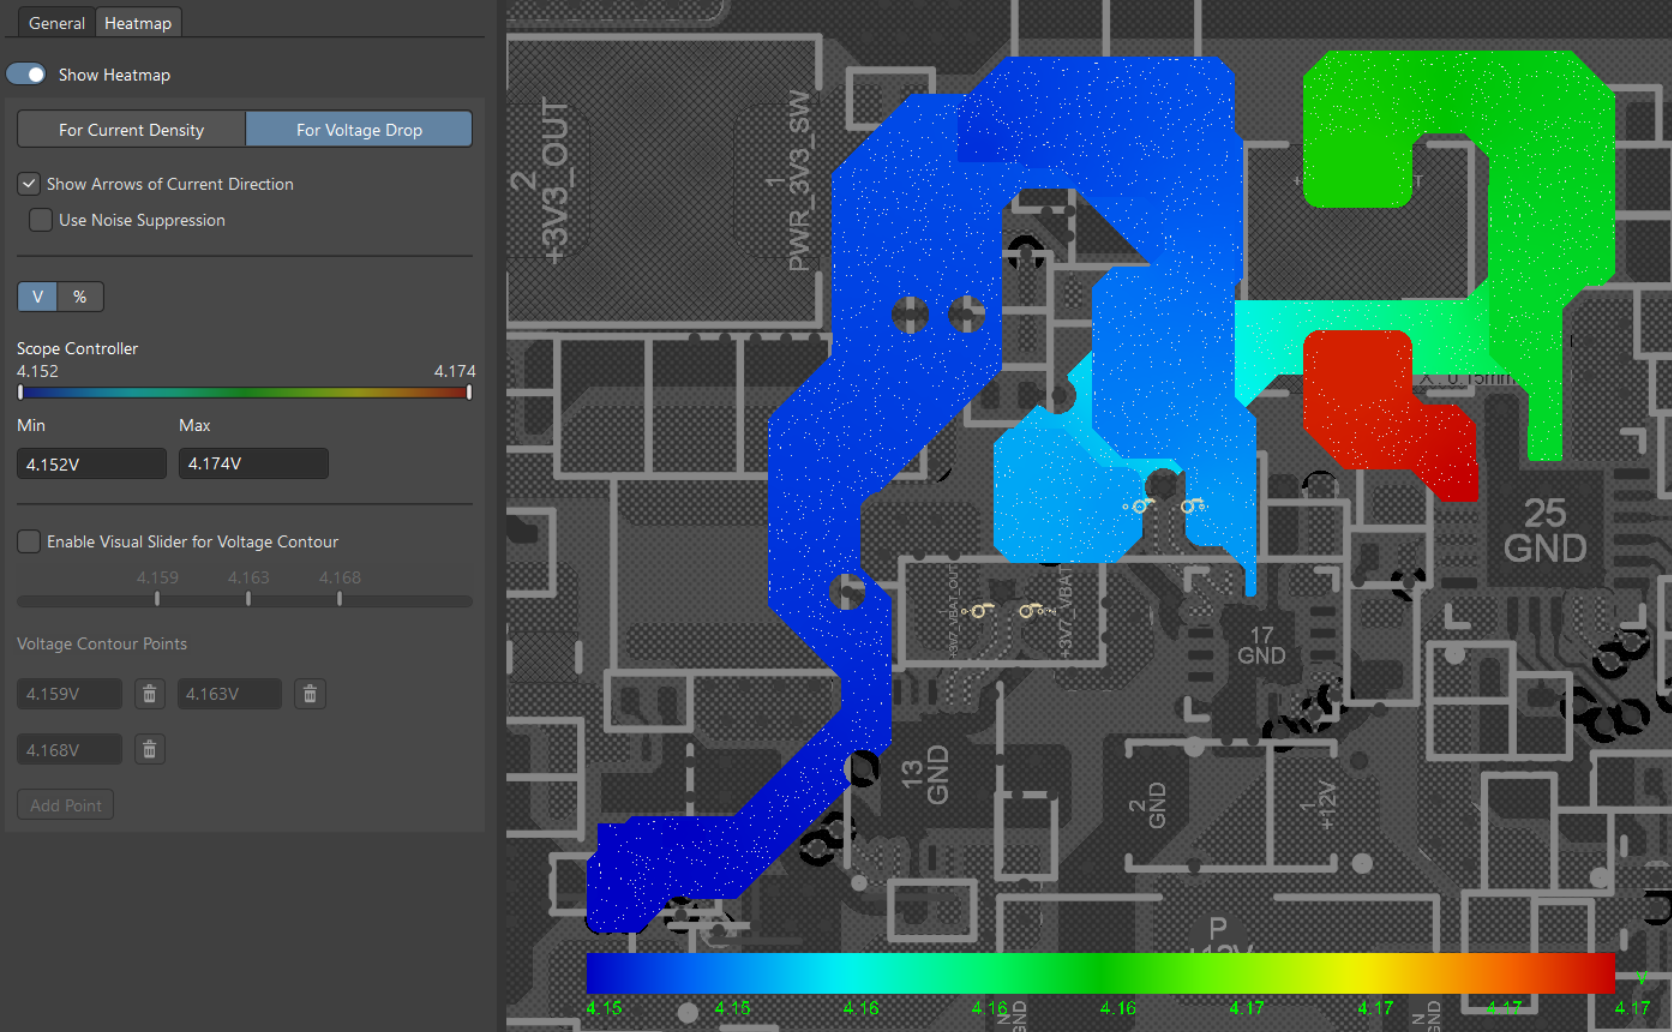
\includegraphics[width=0.6\textwidth]{figures/4v2_vsys_sim_voltage_drop.png}
                        \caption{Biểu đồ phân bố điện áp (Voltage Drop Heatmap) trên nguồn +4V2\_VSYS.}
                        \label{fig:4v2_vsys_voltage_drop}
                    \end{figure}
                    
                    \textbf{\textit{Tính toán lý thuyết:}}


                    \textbf{\textit{Kết quả mô phỏng Sụt áp:}}

                    \begin{itemize}
                        \item Điện áp tại điểm nguồn: $V_{source} = 4.072 V$.
                        \item Điện áp tại điểm tải xa nhất: $V_{load} = 3.96 V$.
                        \item Chênh lệch điện áp: $\Delta V = 4.072V - 3.96V = 112mV$.
                    \end{itemize}

                    \textbf{\textit{Đánh giá:}}
                    \begin{itemize}
                        \item Phần trăm sụt áp so với mức danh định (4.2V): $\%Drop = \dfrac{4.2V - 4.072V}{4.2V} = \mathbf{3.05\%}$\par
                        $\Rightarrow$ Kết quả nhỏ hơn giới hạn 5\%.
                        
                        \item Điện trở đường dẫn: $R_{path} = \dfrac{V_{source} - V_{load}}{I_{load}} = \dfrac{112mV}{4.75A} \approx \mathbf{23.58 m\Omega}$\par
                        $\Rightarrow$ Trở kháng đường dây rất thấp, cho thấy thiết kế layout nguồn tốt.
                    \end{itemize}

                \item \textbf{Phân tích Ray nguồn +5V0:}
                    
                    Mô phỏng được thực hiện với dòng tải tiêu thụ cực đại trên thiết kế là $I_{load} = 2.46A$.
                    
                    \begin{figure}[h]
                        \centering
                        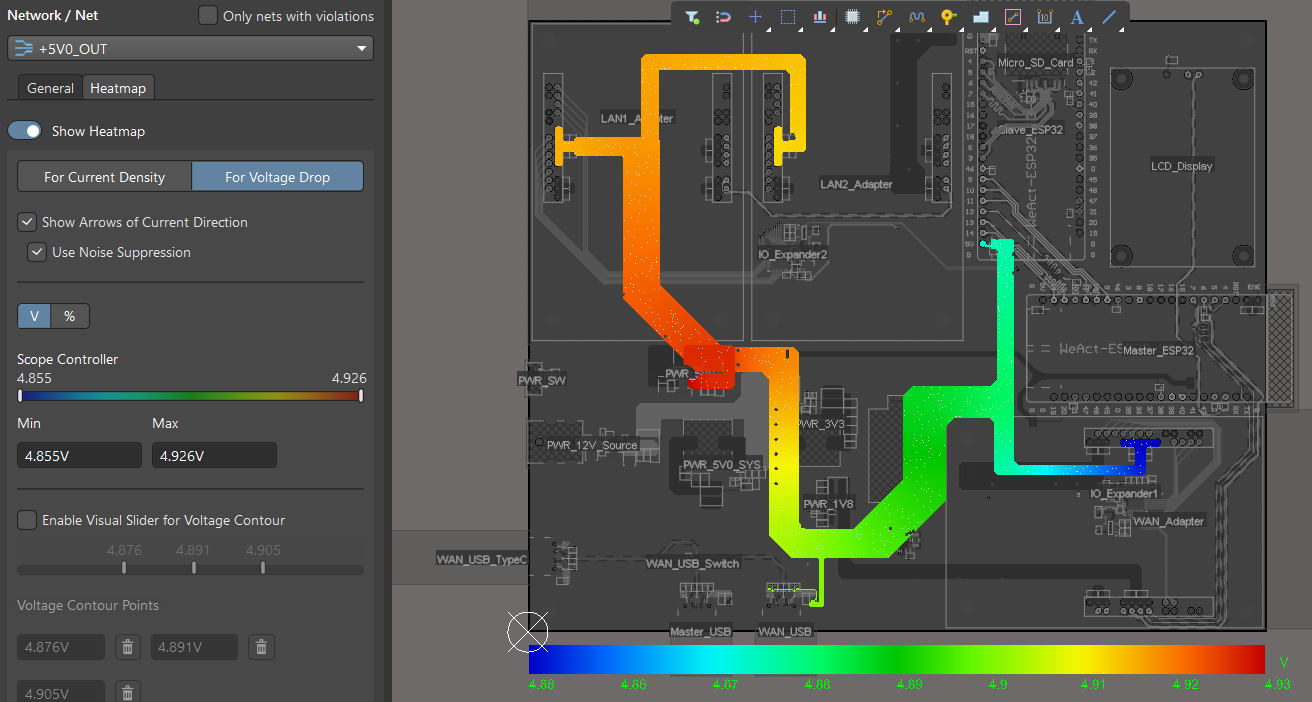
\includegraphics[width=0.55\textwidth]{figures/5v0_sim_voltage_drop.png}
                        \caption{Biểu đồ phân bố điện áp (Voltage Drop Heatmap) trên nguồn +5V0.}
                        \label{fig:5v0_drop}
                    \end{figure}
                    
                    \textbf{\textit{Kết quả mô phỏng và Tính toán:}}
                    \begin{itemize}
                        \item Điện áp tại điểm nguồn: $V_{source} = 4.926 V$.
                        \item Điện áp tại điểm tải xa nhất: $V_{load} = 3.163 V$.
                        \item Chênh lệch điện áp: $\Delta V = 4.926V - 3.163V = 71mV$.
                    \end{itemize}

                    \textbf{\textit{Đánh giá:}}
                    \begin{itemize}
                        \item Phần trăm sụt áp so với mức danh định (5V): $\%Drop = \dfrac{5V - 3.163V}{5V} = \mathbf{2.9\%}$\par
                        $\Rightarrow$ Kết quả nhỏ hơn giới hạn 5\%.
                        
                        \item Điện trở đường dẫn: $R_{path} = \dfrac{V_{source} - V_{load}}{I_{load}} = \dfrac{71mV}{2.46A} \approx \mathbf{2.89 m\Omega}$\par
                        $\Rightarrow$ Trở kháng đường dây rất thấp, cho thấy thiết kế layout nguồn tốt.
                    \end{itemize}

                \item \textbf{Phân tích Ray nguồn +3V3:}
                    
                    Mô phỏng được thực hiện với dòng tải tiêu thụ cực đại trên thiết kế là $I_{load} = 3.3A$.
                    
                    \begin{figure}[h]
                        \centering
                        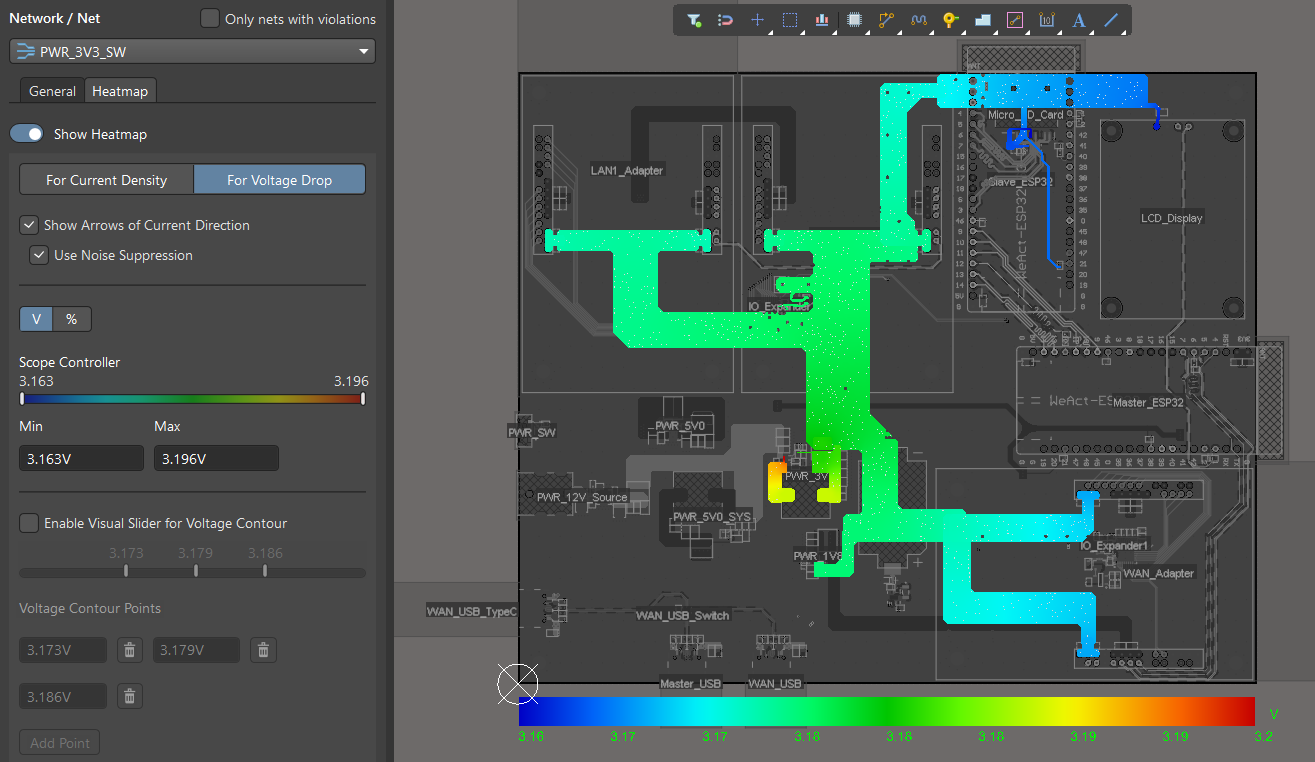
\includegraphics[width=0.55\textwidth]{figures/3v3_sim_voltage_drop.png}
                        \caption{Biểu đồ phân bố điện áp (Voltage Drop Heatmap) trên nguồn +3V3.}
                        \label{fig:3v3_drop}
                    \end{figure}
                    
                    \newpage
                    \textbf{\textit{Kết quả mô phỏng và Tính toán:}}
                    \begin{itemize}
                        \item Điện áp tại điểm nguồn: $V_{source} = 3.196 V$.
                        \item Điện áp tại điểm tải xa nhất: $V_{load} = 3.163 V$.
                        \item Chênh lệch điện áp: $\Delta V = 3.196V - 3.163V = 33mV$.
                    \end{itemize}

                    \textbf{\textit{Đánh giá:}}
                    \begin{itemize}
                        \item Phần trăm sụt áp so với mức danh định (3.3V): $\%Drop = \dfrac{3.3V - 3.163V}{3.3V} = \mathbf{4.15\%}$\par
                        $\Rightarrow$ Kết quả tuy nhỏ hơn nhưng khá gần giới hạn 5\%.
                        
                        \item Điện trở đường dẫn: $R_{path} = \dfrac{V_{source} - V_{load}}{I_{load}} = \dfrac{33mV}{3.3A} \approx \mathbf{10 m\Omega}$\par
                        $\Rightarrow$ Trở kháng đường dây rất thấp, cho thấy thiết kế layout nguồn tốt. Song mức sụt áp khá gần giới hạn, cho thấy sụt áp xảy ra tại nguồn là khá cao.
                    \end{itemize}
            \end{enumerate}


        \subsubsection{Phân tích và Mô phỏng Mật độ dòng điện (Current Density Analysis)}

            Bên cạnh sụt áp, mật độ dòng điện là tham số quan trọng quyết định độ bền vật lý của bo mạch. Mật độ dòng quá cao sẽ gây ra hai vấn đề:
            \begin{itemize}
                \item \textbf{Quá nhiệt (Overheating):} Công suất tiêu tán tập trung tại một điểm nhỏ có thể nung nóng đường mạch, làm bong tróc lớp đồng hoặc hỏng lớp cách điện PCB.
                \item \textbf{Giảm hiệu suất và tăng nhiễu điện từ:} Mật độ dòng cao làm tăng điện trở gây sụt áp, ngoài ra với dòng chuyển mạch nhanh, mật độ dòng quá lớn gây ra tác động EMI mạnh mẽ hơn.
            \end{itemize}

            \textbf{Tiêu chí thiết kế:}
            \begin{itemize}
                \item Tuân thủ tiêu chuẩn IPC-2221: Mức tăng nhiệt độ tối đa $\Delta T \le 10^\circ C$.
                \item Ngưỡng mật độ dòng điện trung bình an toàn: $J_{avg} \le 50 A/mm^2$ (đối với lớp đồng 1oz).
            \end{itemize}

            \begin{enumerate}
                \renewcommand{\labelenumi}{\alph{enumi}.}
                \item \textbf{Phân tích Ray nguồn +5V0\_SYS:}
                    
                    Mô phỏng được thực hiện với dòng tải tiêu thụ cực đại trên thiết kế là $I_{load} = 2.92A$.

                    \begin{figure}[h]
                        \centering
                        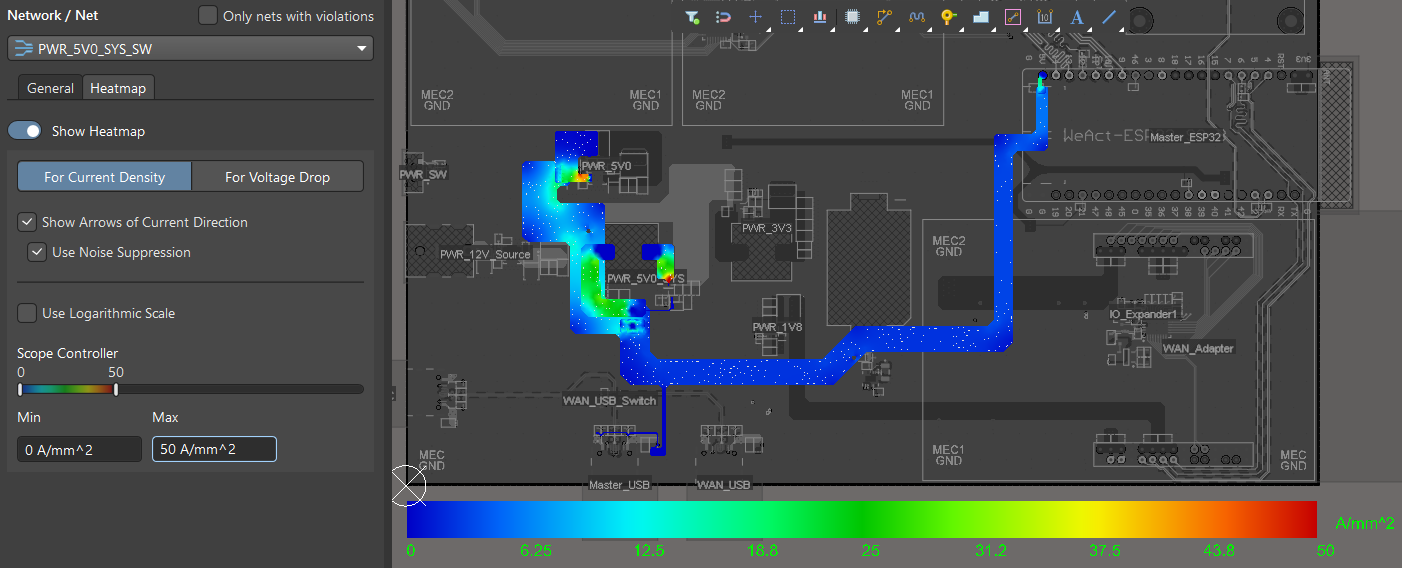
\includegraphics[width=0.6\textwidth]{figures/5v0_sys_sim_current_density.png}
                        \caption{Biểu đồ phân bố mật độ dòng điện (Current Density Heatmap) trên nguồn +5V0\_SYS.}
                        \label{fig:5v0_sys_current_density}
                    \end{figure}

                    \textbf{\textit{Kết quả tổng thể:}}
                    Quan sát \autoref{fig:5v0_sys_current_density}, mật độ dòng điện trên phần lớn chiều dài đường mạch được duy trì ở mức thấp (màu xanh dương/xanh lá), nằm hoàn toàn trong ngưỡng an toàn ($< 30 A/mm^2$). Điều này xác nhận kích thước các đường nguồn đã được thiết kế đủ rộng.

                    \textbf{\textit{Phân tích điểm có mật độ dòng điện cao đột biến:}}
                    
                    \begin{figure}[h]
                        \centering
                        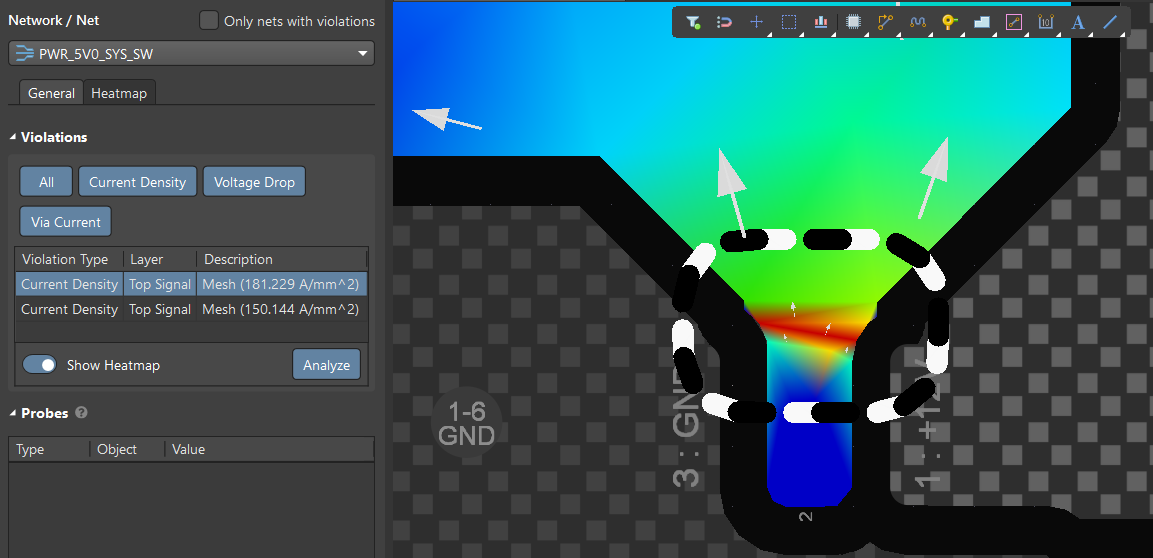
\includegraphics[width=0.6\textwidth]{figures/5v0_sys_sim_current_density_high.png}
                        \caption{Mật độ dòng điện cao đột biến tại pinout nguồn xung +5V0\_SYS.}
                        \label{fig:5v0_sys_current_density_high}
                    \end{figure} 

                    Tại vị trí pinout của IC nguồn xung (\autoref{fig:5v0_sys_current_density_high}), ghi nhận mật độ dòng điện tăng vọt lên mức khá cao $J \approx 181.229 A/mm^2$. Mặc dù giá trị này vượt ngưỡng an toàn, nhưng thiết kế vẫn được đảm bảo:
                    \begin{itemize}
                        \item Mật độ cao chỉ xuất hiện tại tiết diện rất nhỏ ngay pinout linh kiện. Đây là giới hạn vật lý của linh kiện mà không thể can thiệp bằng layout. Với tiết diện đoạn mạch chịu dòng cao là cực nhỏ ($< 0.25mm \times 0.45 mm$), rủi ro về sụt áp là không đáng kể.
                        \item Ngay sau điểm đó, đường mạch lập tức được mở rộng thành mảng đồng lớn. Nhiệt lượng sinh ra tại điểm này sẽ nhanh chóng được dẫn truyền và tản ra khu vực đồng xung quanh, ngăn chặn việc tăng nhiệt độ quá mức.
                    \end{itemize}

                \item \textbf{Phân tích Ray nguồn +5V0:}
                    
                    Mô phỏng được thực hiện với dòng tải tiêu thụ cực đại trên thiết kế là $I_{load} = 2.46A$.

                    \begin{figure}[h]
                        \centering
                        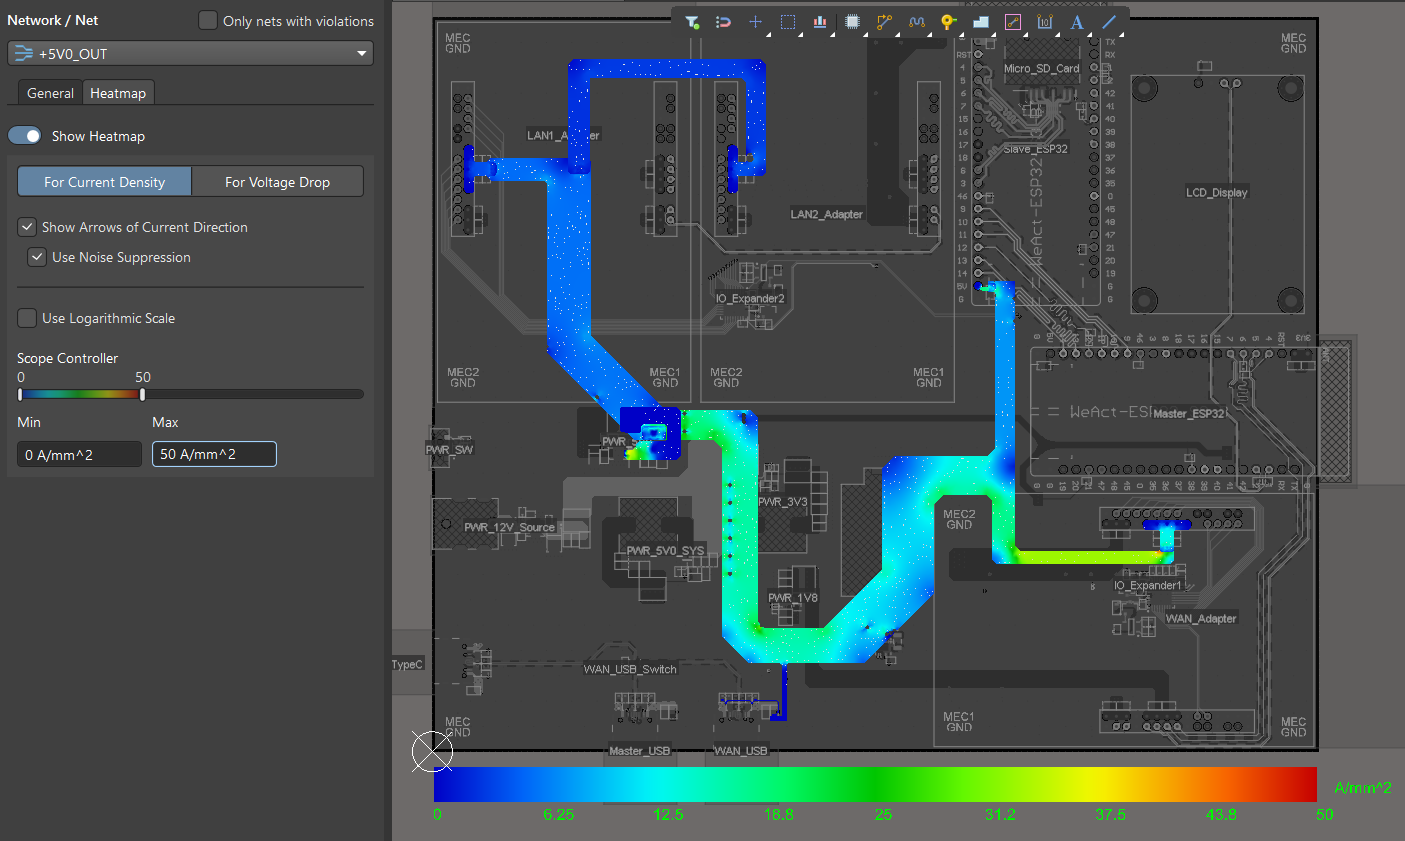
\includegraphics[width=0.6\textwidth]{figures/5v0_sim_current_density.png}
                        \caption{Biểu đồ phân bố mật độ dòng điện (Current Density Heatmap) trên nguồn +5V0.}
                        \label{fig:5v0_current_density}
                    \end{figure}

                    \textbf{\textit{Kết quả tổng thể:}}
                    Quan sát \autoref{fig:5v0_current_density}, mật độ dòng điện trên phần lớn chiều dài đường mạch được duy trì ở mức thấp (màu xanh dương/xanh lá), nằm hoàn toàn trong ngưỡng an toàn ($< 30 A/mm^2$). Điều này xác nhận kích thước các đường nguồn đã được thiết kế đủ rộng.                            

                \item \textbf{Phân tích Ray nguồn +3V3:}
                    
                    Mô phỏng được thực hiện với dòng tải tiêu thụ cực đại trên thiết kế là $I_{load} = 3.3A$.

                    \begin{figure}[h]
                        \centering
                        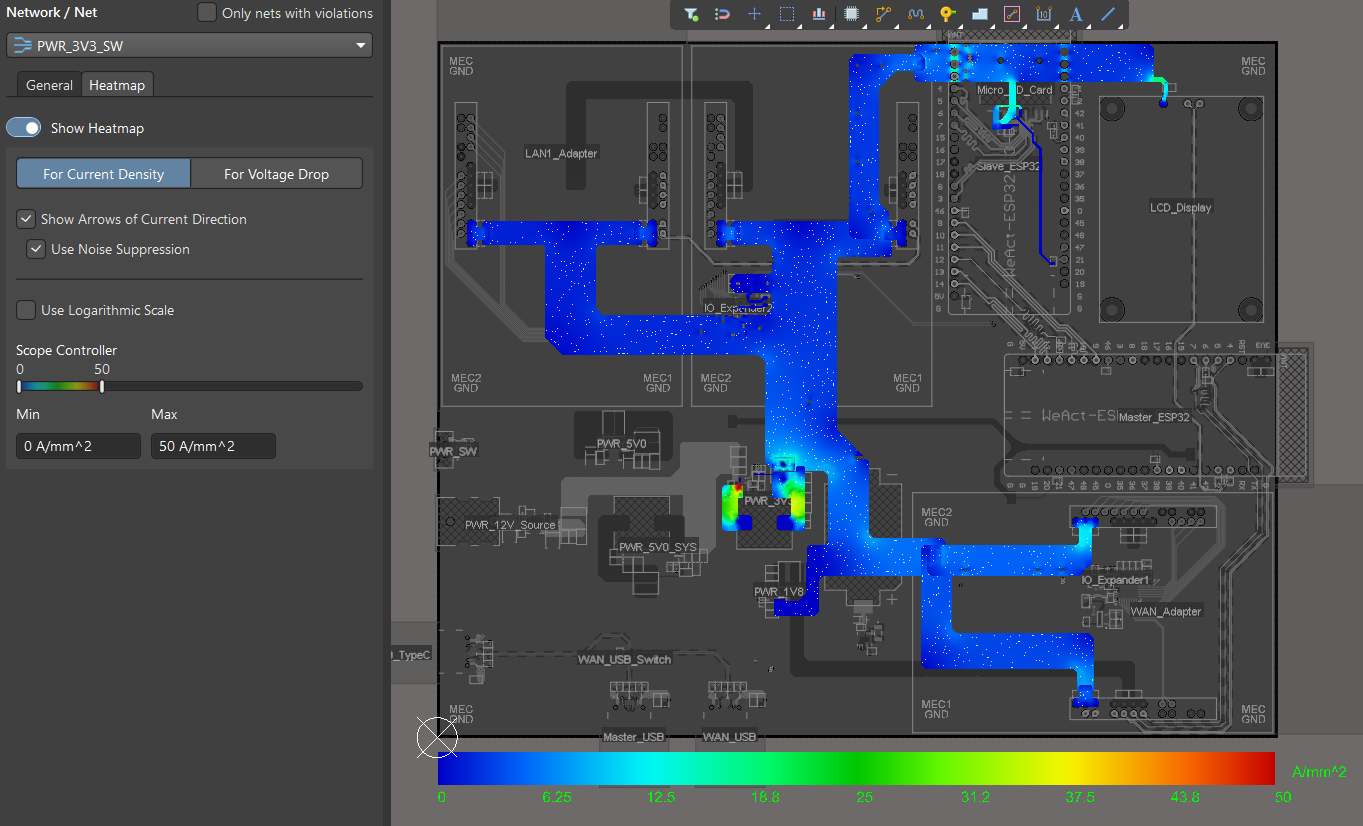
\includegraphics[width=0.6\textwidth]{figures/3v3_sim_current_density.png}
                        \caption{Biểu đồ phân bố mật độ dòng điện (Current Density Heatmap) trên nguồn +3V3.}
                        \label{fig:3v3_current_density}
                    \end{figure}

                    \textbf{\textit{Kết quả tổng thể:}}
                    Quan sát \autoref{fig:3v3_current_density}, mật độ dòng điện trên phần lớn chiều dài đường mạch được duy trì ở mức thấp (màu xanh dương/xanh lá), nằm hoàn toàn trong ngưỡng an toàn ($< 30 A/mm^2$). Điều này xác nhận kích thước các đường nguồn đã được thiết kế đủ rộng.

                    \textbf{\textit{Phân tích điểm có mật độ dòng điện cao đột biến:}}
                    
                    \begin{figure}[h]
                        \centering
                        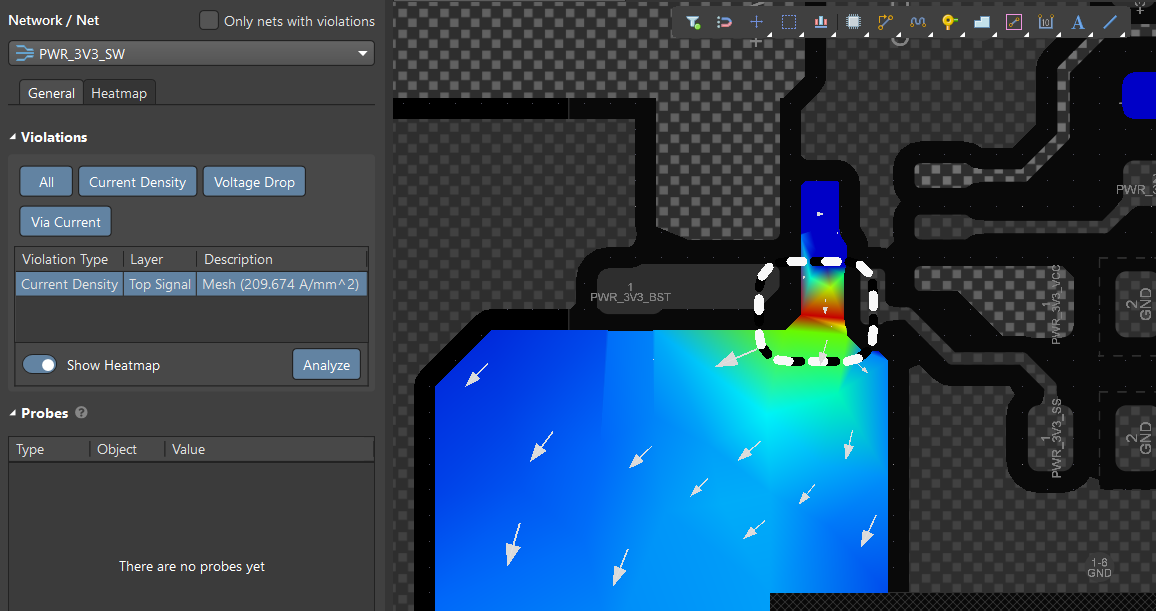
\includegraphics[width=0.6\textwidth]{figures/3v3_sim_current_density_high.png}
                        \caption{Mật độ dòng điện cao đột biến tại pinout nguồn xung +3V3.}
                        \label{fig:3v3_current_density_high}
                    \end{figure} 

                    Tương tự với nguồn +5V0\_SYS, tại vị trí pinout của IC nguồn xung (\autoref{fig:3v3_current_density_high}), ghi nhận mật độ dòng điện tăng vọt lên mức khá cao $J \approx 209.674 A/mm^2$. Mặc dù giá trị này vượt ngưỡng an toàn, nhưng thiết kế vẫn được đảm bảo.
            \end{enumerate}

